\subsection{Specifikace požadavků}
Specifikace a analýza požadavků je první fáze vývoje softwaru. \textbf{Cílem je definovat požadavky na software a popsat jeho funkcionalitu}. Výsledkem této fáze by měly být dokumenty, které se stanou součásti smlouvy mezi zadavatelem a vývojovým týmem. \textbf{Kvalita} výsledného produktu je pak dána \textbf{mírou uspokojení požadavků zadavatele}.

V rámci specifikace požadavků je třeba analyzovat procesy u zadavatele, které bude software řešit, nebo s ním nějak jinak souvisí. K popisu těchto procesů dobře poslouží \textbf{Diagram případu užití}, \textbf{Sekvenční diagram} a \textbf{Diagram aktivit}.

\subsubsection{Cíle požadavků}
\begin{itemize}
\item chceme vytvořit a udržovat dohody se zákazníky a dalšími zainteresovanými stranami o tom, co by \textbf{systém měl dělat a proč},
\item aby vývojáři lépe pochopili \textbf{požadavky na systém},
\item definování \textbf{hranic systému},
\item vytvořit základ pro plánování \textbf{technického obsahu} interakcí,
\item poskytnout základ pro \textbf{odhad} \textbf{nákladů} a \textbf{času} na \textbf{vytvoření systému},
\item definovat \textbf{uživatelské rozhraní} pro systém, se zaměřením na potřeby uživatelů.
\end{itemize}

\subsubsection{Aktivity spojené s analýzou požadavků}
\begin{itemize}
	\item \textbf{Sběr požadavků} --  komunikace se zákazníky a uživateli za účelem získání jejich požadavků na systém.
	\item \textbf{Analýza požadavků} -- identifikování nejasných požadavků, nekompletních, nebo protichůdných a následné řešení těchto nesrovnalostí.
	\item \textbf{Zaznamenání požadavků} -- dokumentování požadavků v různých formách, jako běžný textový dokument, případy užití (use case), nebo specifikace procesů.
\end{itemize}
Požadavky je také nutno: \textbf{organizovat}, \textbf{dokumentovat}, \textbf{priorizovat}, \textbf{filtrovat} a \textbf{sledovat}.

\subsubsection{Typy požadavků -- FURPS}
\begin{itemize}
\item \textbf{Funkční požadavky (chování)} -- se používají k vyjádření chování systému zadáním jak vstupních tak i výstupních podmínek.
\item \textbf{Doplňující požadavky (nefunkční)}
\begin{itemize}
\item \textbf{Použitelnost (Usability)} -- se zabývá lidskými faktory, jako je vzhled, snadné používání, atd.
\item \textbf{Spolehlivost (Reliability)} --  četnost a závažnost selhání, obnovitelnost a přesnost.
\item \textbf{Výkon (Performance)} -- se zabývá množstvím transakcí, jako je rychlost, doba odezvy, atd.
\item \textbf{Podporovatelnost (Supportability)} -- řeší, jak těžké je udržet systém a další vlastnosti potřebné k udržení systému po jeho vydání.
\end{itemize}
\end{itemize}

\subsection{Diagram případů užití}
\textbf{Případ užití (use case)} -- je technika pro zdokumentování případného požadavku na nový systém, nebo změny na stávající systém. Každý use case poskytuje jeden nebo více scénářů, které zaznamenávají, jak by systém měl spolupracovat s koncovým uživatelem nebo jiným systémem.

Diagram případu užití popisuje \textbf{vztahy} mezi \textbf{aktéry} a jednotlivými \textbf{případy užití}. Součástí diagramu jsou:
\begin{itemize}
\item \textbf{Aktéři} -- definují \textbf{uživatele} či \textbf{jiné systémy}, kteří budou vstupovat do interakce s vyvíjeným softwarovým systémem.
\item \textbf{Relace (vztahy)} -- \textbf{vazby} a \textbf{vztahy} mezi aktéry a případy užití. V diagramu jsou znázorněny \textbf{šipkami případně čárami}.
\item \textbf{Případy užití} -- specifikující vzory chování  softwarovým systémem.  Každý případ užití lze chápat jako \textbf{posloupnost vzájemně navazujících transakcí} vykonaných \textbf{v dialogu mezi aktérem a vlastním softwarovým systémem}.
\item \textbf{Scénář} -- unikátní sekvence akcí skrz use-case (jedna cesta/instance provedení).
\end{itemize}
\textbf{Účelem} diagramu případů užití \textbf{je definovat co existuje vně vyvíjeného systému} (\textbf{aktéři}) a \textbf{co má být systémem prováděno (případy užití)}. Vstupem pro sestavení diagramu případů užití je \textbf{byznys model}, konkrétně modely podnikových procesů.  \textbf{Výsledkem} analýzy těchto procesů \textbf{je seznam požadovaných funkcí softwarového systému}, které podpoří nebo dokonce nahradí některé z uvedených aktivity jejich softwarovou implementací.

\begin{figure}[H]
	\centering
	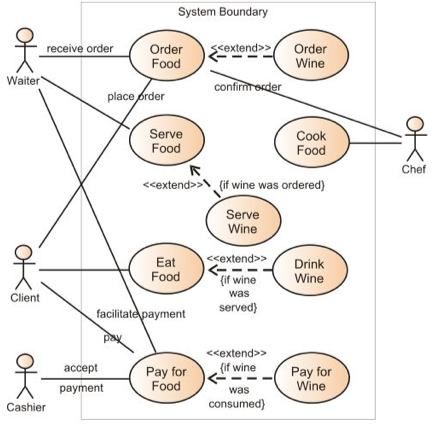
\includegraphics[width=0.7\textwidth]{assets/usecase.png}
\end{figure}

\noindent Pro složitější a obsáhlejší diagramy případů užití se zavadí \textbf{tři (+1) typy vztahů}:
\begin{itemize}
    \item \textbf{Relace} - bez typu (jen čára) značí přístup k UC, nejčastěji mezi aktéri a UC
\item \textbf{Include} – případ užití musí \textbf{obsahovat} jiný (UC s include se vždy provede před samotným UC).
\item \textbf{Extend} – případ užití může \textbf{rozšiřovat} jiný (UC s extend se může nebo nemusí provést).
\item \textbf{Generalizace} – případ užití může být \textbf{speciálním případem} jiného (dědičnost).
\end{itemize}

\subsubsection{Doporučená forma vytváření use-case}
\begin{itemize}
\item má vyjadřovat \textbf{co systém dělá} (ne jak) a co od něj očekávají aktéři,
\item měly by být používány jen pojmy problémové domény -- žádné neznámé termíny,
\item případy užití by měly být co \textbf{nejjednodušší}, ať jim rozumí i zadavatelé -- nepoužívat příliš \texttt{<include>} a \texttt{<extend>},
\item \textbf{nepoužívat} příliš funkční dekompozici (\textbf{specializaci}),
\item primární aktéři umístěni vlevo a pojmenováni krátkým podstatným jménem,
\item každý \textbf{aktér} by měl být \textbf{propojen s minimálně jedním use-case},
\item základní use case vlevo a další kreslit směrem doprava, rozšířující use-case směrem dolů.
\end{itemize}

\subsection{Sekvenční diagram}
Sekvenční diagram popisuje funkce systému z pohledu \textbf{objektů} a\textbf{ jejich interakcí}. Komunikace mezi objekty je \textbf{znázorněná v čase}, takže z diagramu můžeme vyčíst i životní cyklus objektu. 

Tento diagram popisuje jaké \textbf{zprávy} (\textbf{požadavky}) \textbf{jsou mezi objekty zasílány} \textbf{z pohledu času}. Diagram je tvořen \textbf{objekty uspořádanými do sloupců} a šipky mezi nimi odpovídají {vzájemně si zasílaným zprávám}. Zprávy mohou být {synchronní} nebo {asynchronní}. V případě \textbf{synchronních zpráv odesílatel čeká na odpověď} (odezvu) adresáta, v případě \textbf{asynchronní zprávy odesílatel nečeká} na odpověď a pokračuje ve vykonávání své činnosti. Souvislé provádění nějaké činnosti se v sekvenčním diagram vyjadřuje svisle orientovaným obdélníkem. Odezvu adresáta lze opět modelovat, v tomto případě tzv. \textbf{návratovou zprávou (přerušovaná čára)}. Tok času probíhá ve směru od shora dolů.
\\\\
\noindent\makebox[\textwidth]{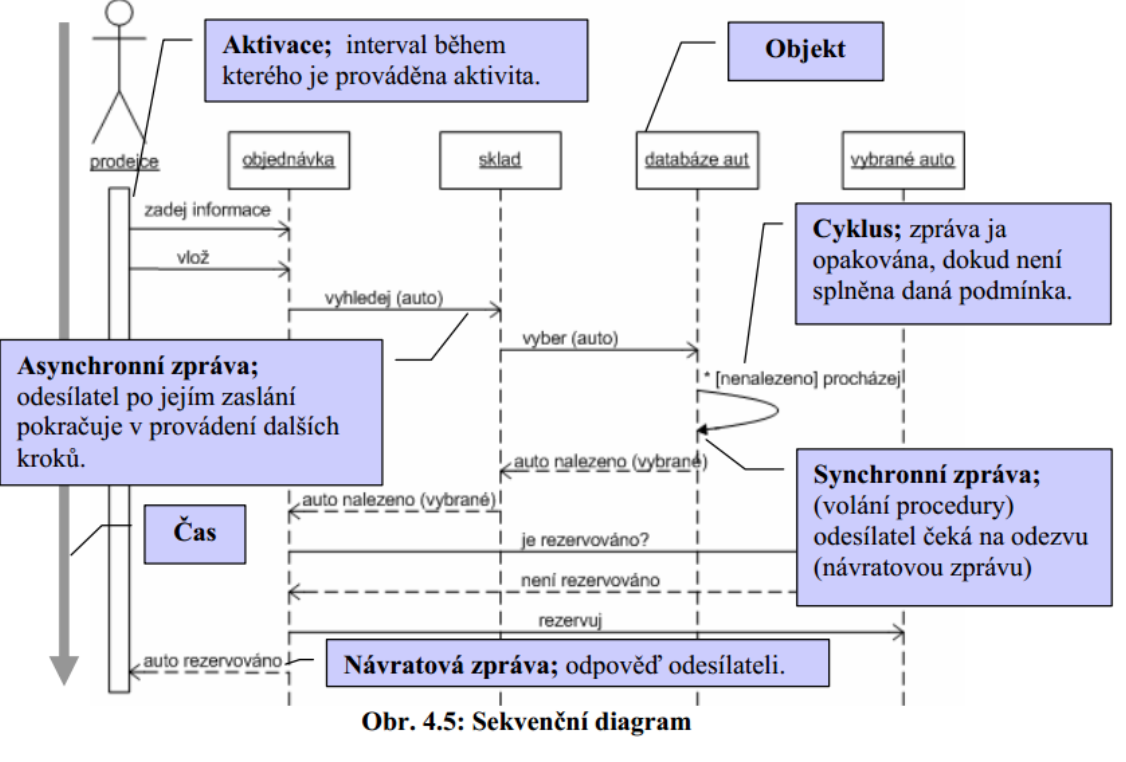
\includegraphics[width=1\textwidth]{assets/sekv}}

\pagebreak
\subsection{Diagram aktivit}
Diagram aktivit popisuje jednotlivé procesy pomocí aktivit reprezentující jeho (akční) \textbf{stavy} a \textbf{přechody mezi nimi}. Pokud aktivita "přetéká" v jednotlivých stavech mezi uživateli, mohou být tyto stavy naznačeny pomocí tzv \textbf{swimlines}.
\begin{figure}[H]
    \centering
    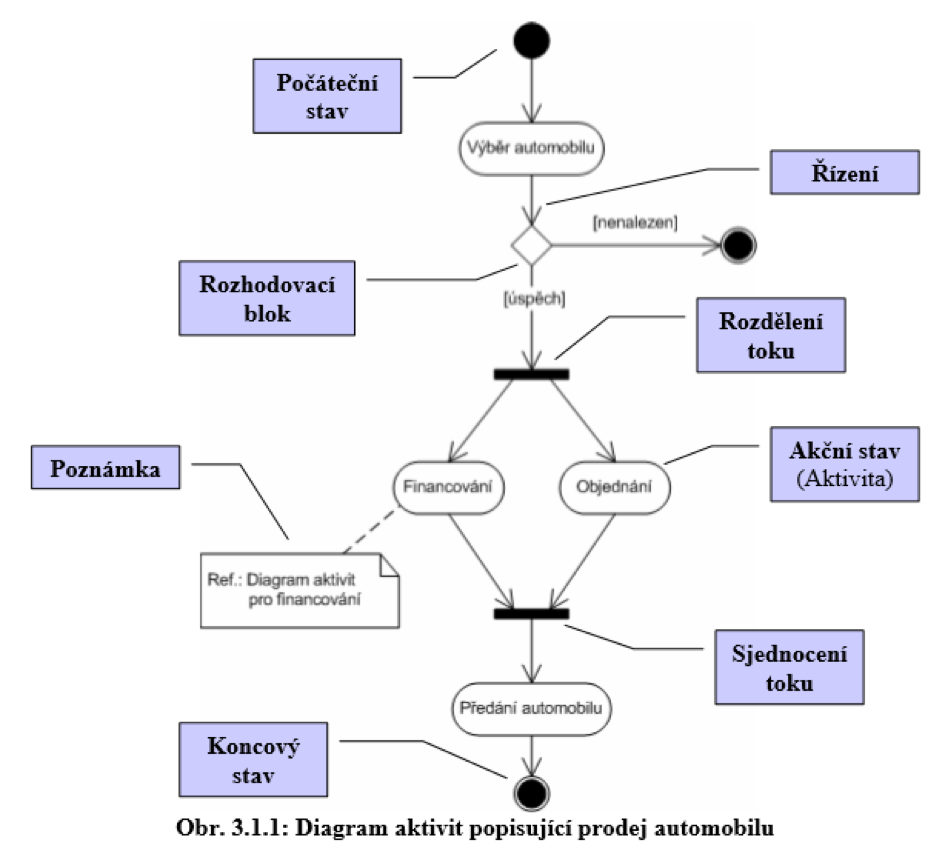
\includegraphics[width=0.9\textwidth]{assets/diag_aktivit.png}
\end{figure}

\begin{figure}[H]
	\centering
	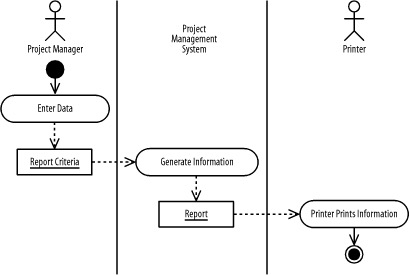
\includegraphics[width=0.6\textwidth]{assets/diag_aktivit_swimlines}
\end{figure}